\section{The fixed \texorpdfstring{$A_3/S_4$}{A3/S4} model}\label{sec:model}

\subsection{The tetrahedron and its Coxeter chambers}

Let
\[
 H=\left\{x\in\mathbb R^4:\sum_{i=0}^{3}x_i=1\right\},
 \qquad
 T=\operatorname{conv}\{e_0,e_1,e_2,e_3\}\subset H,
\]
with the induced Euclidean metric.  This is a regular tetrahedron of edge
length $\sqrt2$; rescaling does not affect any statement below.  For a
nonempty set $I\subseteq\{0,1,2,3\}$ put
\[
 b_I=\frac1{|I|}\sum_{i\in I}e_i.
\]
If $\sigma=\sigma_0\sigma_1\sigma_2\sigma_3$ is a one-line permutation, the
closed barycentric chamber indexed by $\sigma$ is
\[
 \Delta_\sigma=
 \operatorname{conv}\left(
 b_{\{\sigma_0\}},
 b_{\{\sigma_0,\sigma_1\}},
 b_{\{\sigma_0,\sigma_1,\sigma_2\}},
 b_{\{0,1,2,3\}}
 \right).
\]
The $24$ chambers have disjoint interiors and union $T$.

Write $G=S_4$.  We compose permutations as functions,
$(pq)(i)=p(q(i))$.  The coordinate permutation
\[
 \Phi_g(x)_i=x_{g^{-1}(i)}
\]
is an isometry of $T$ and satisfies
$\Phi_g(\Delta_\sigma)=\Delta_{g\sigma}$.  Hence the full isometry group of
$T$ is realised by left multiplication on chamber labels; its
orientation-preserving subgroup is $A_4$.

Let $s_i$ exchange positions $i$ and $i+1$ for $i=0,1,2$.  Two chambers
share a facet precisely when their labels differ by right multiplication by
one $s_i$.  The chamber graph is therefore
\[
 \Gamma=\operatorname{Cay}_{\mathrm{right}}
 (S_4,\{s_0,s_1,s_2\}).
\]
Left multiplication is a graph automorphism because
$g(\sigma s_i)=(g\sigma)s_i$.

\begin{figure}[ht]
\centering
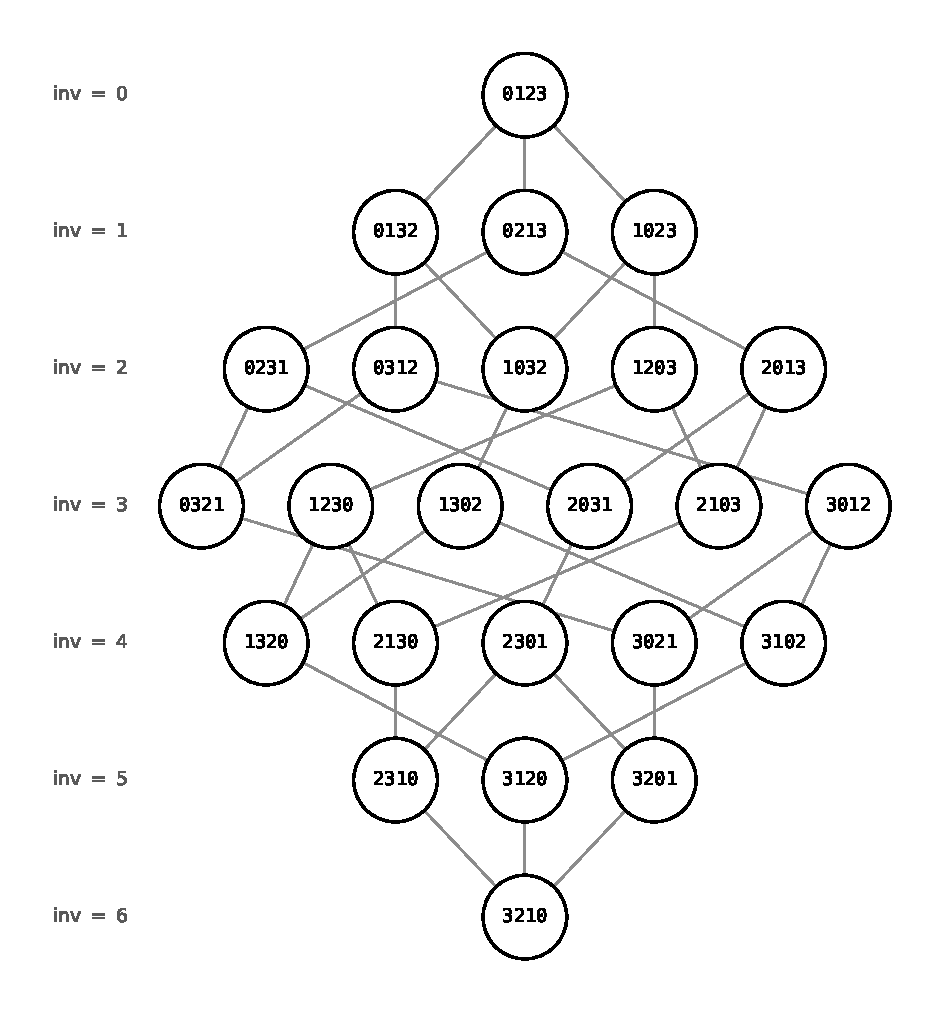
\includegraphics[width=.72\textwidth]{figures/a3_chamber_graph.pdf}
\caption{The $24$ chambers and their facet-adjacency graph.  Edges are
right multiplication by an adjacent transposition; left $S_4$ acts by graph
automorphisms.  Figure reused from \cite{BabanskyyT2} under CC BY 4.0.}
\label{fig:chamber-graph}
\end{figure}

\subsection{Pieces, masks, and convexity}

\begin{definition}[Coxeter-pure piece]
A piece is a nonempty subset $U\subseteq G$, identified with the closed
polyhedron
\[
 |U|_T=\bigcup_{\sigma\in U}\Delta_\sigma.
\]
It is \emph{connected} when the induced chamber graph $\Gamma[U]$ is
connected.  This is facet-connectedness; contact through only an edge or a
vertex does not suffice.
\end{definition}

Order the $24$ words lexicographically and let $\operatorname{idx}(\sigma)$
be the zero-based position.  The integer mask
\[
 m(U)=\sum_{\sigma\in U}2^{\operatorname{idx}(\sigma)}
\]
is the primary exact encoding.  All masks in the paper are displayed as six
hexadecimal digits.

For $i,j\in\{0,1,2,3\}$ define $i<_{U}j$ when $i$ precedes $j$ in every word
of $U$.  These unanimous precedence relations define a poset $P_U$.  Its set
of linear extensions is the halfspace closure
\[
 \operatorname{hcl}(U)=L(P_U).
\]
We call $U$ halfspace-convex when $U=\operatorname{hcl}(U)$ and
halfspace-nonconvex otherwise.  For connected pieces this agrees with
chamber-geodesic and Euclidean convexity by the three-way theorem of
\cite{BabanskyyT2}.  The computation uses the halfspace predicate; the
geometric terminology invokes that theorem with its stated hypotheses.

\subsection{Four typed equivalences}

\begin{definition}[Tile orbit]
The left tile orbit and stabiliser of $U$ are
\[
 \Orb_L(U)=\{gU:g\in G\},
 \qquad H_U=\Stab_L(U)=\{g\in G:gU=U\}.
\]
Two pieces are \emph{left-tile equivalent} when they lie in the same
$\Orb_L$ orbit.  The canonical representative is
\[
 \can_L(U)=\arg\min_{V\in\Orb_L(U)}m(V).
\]
The minimum is numeric bitmask order, not lexicographic order on word lists.
\end{definition}

\begin{definition}[Exact cover]
An exact left-translate cover of $U$ is an unordered set
\[
 \C=\{g_1U,\ldots,g_rU\}\subseteq\Orb_L(U)
\]
whose chamber sets are pairwise disjoint and whose union is $G$.  Necessarily
$r=24/|U|$.  Covers $\C$ and $\C'$ are \emph{cover equivalent} when
$\C'=g\C:=\{gV:V\in\C\}$ for one $g\in G$.
\end{definition}

\begin{definition}[Selector]
A multiplier selector for a cover $\C$ of $U$ is a set $A\subseteq G$ such
that
\[
 \C=\{aU:a\in A\}.
\]
Selectors are not unique when $H_U$ is nontrivial.  Their natural global-left
action is $A\mapsto gA$.
\end{definition}

\begin{definition}[Free congruence]
Pieces $U,V$ are \emph{freely congruent} if an affine Euclidean isometry of
$H$ maps $|U|_T$ onto $|V|_T$.  This does not, by definition, require the
isometry to preserve the ambient tetrahedron.  Whole partitions are
congruent when one isometry of $H$ maps the complete unordered family of
pieces onto the other.
\end{definition}

\begin{definition}[Congruent Coxeter-pure cover]
A congruent Coxeter-pure cover is an unordered family
$\{U_1,\ldots,U_r\}$ of connected pieces in the fixed chamber carrier whose
polyhedral interiors are pairwise disjoint, whose union is $T$, and whose
members are pairwise freely congruent.  Thus every member is itself a union
of chambers of the fixed $A_3$ dissection.  This is the finite-carrier
meaning of \emph{by congruent copies} used in the Coxeter-pure problem;
copies whose boundaries cut chamber interiors are outside the definition.
\end{definition}

The first three definitions are finite group actions.  Free congruence is a
geometric relation and must be compared with them rather than identified by
notation.  Right multiplication is also distinct: it conjugates the
adjacent-transposition generating set and need not preserve connectivity.

\begin{lemma}[Basic covariance]\label[lemma]{lem:basic-covariance}
Left multiplication preserves chamber adjacency, cardinality, halfspace
closure, exact-cover incidence, and Euclidean shape.  Moreover
\[
 |\Orb_L(U)|=\frac{24}{|H_U|}.
\]
\end{lemma}
\begin{proof}
Adjacency covariance was observed above.  Relabelling the ground set carries
the precedence poset $P_U$ to $P_{gU}$, so it carries their linear extensions
and halfspace closures.  The other assertions follow from the coordinate
isometry $\Phi_g$, and the final identity is orbit--stabiliser.
\end{proof}
